
%%%%%%%%%%%%%%%%%%%%%%%%%%%%%%%%%%%%%%%%%%%%%%%%%%%%%%%%%%%%%%%%%%%%%%%%
%
%		Chapter 1 - Introduction to ODEs
%
%%%%%%%%%%%%%%%%%%%%%%%%%%%%%%%%%%%%%%%%%%%%%%%%%%%%%%%%%%%%%%%%%%%%%%%%


\begin{topic}[Introduction to Differential Equations]

\end{topic}




%%%%%%%%%%%%%%%%%%%%%%%%%%%%%%%%%%%%%%%%%%%%%%%%%%%%%%%%%%%%%%%%%%%%%%%%
%		Definitions


\begin{module}{Definition}
%	\Title{Definitions}
	\Heading{Textbook}	
	\Heading{Objectives}
	\begin{itemize}
		\item Bla bla bla	
	\end{itemize}
	
	\Heading{Motivation} 


\end{module}


















\newpage


%%%%%%%%%%%%%%%%%%%%%%%%%%%%%%
%
%  MODULE - Solutions
%
%%%%%%%%%%%%%%%%%%%%%%%%%%%%%%



\begin{module}{Solutions}
	%\Title{Solutions}
	\label{intro-sols}

	\input{modules/module8-sols.tex}
	\input{modules/module8-sols-exercises.tex}
\end{module}



\begin{lesson}
	\Title{Solutions}

	\Heading{Objectives}
	\begin{itemize}
		\item The second step in Mathematical modelling is to construct a representation of how the team will be attempting to solve the problem.
		\item Create a mind map of the problem. This is a structured way to brainstorm possible solutions and their requirements.
	\end{itemize}
	
	\Heading{Motivation} 

\begin{annotation}
	\begin{goals}
	\Goal{Extra Reading}
	Math Modelling: Getting started and getting solutions, Bliss-Fowler-Galluzzo
	
	\hfill \qrcode{https://m3challenge.siam.org/resources/modeling-handbook}	
	\end{goals}
\end{annotation}
	\Heading{Extra Reading} \href{https://m3challenge.siam.org/resources/modeling-handbook}{Math Modelling: Getting started and getting solutions, Bliss-Fowler-Galluzzo}

\end{lesson}




\newpage

\question

Which of these shows solutions of $y' = (x-1)(x+1) = x^2 - 1$ ?

\newlength{\len}
\setlength{\len}{120pt}
\begin{tabular}{ccc}
\includegraphics[width=\len]{images/module8-figs-6.png}
	& \includegraphics[width=\len]{images/module8-figs-3.png}
	& \includegraphics[width=\len, page=2]{images/module8-figs-2.png} \\
A & B & C \\[15pt]
%
\includegraphics[width=\len]{images/module8-figs-1.png}
	& \includegraphics[width=\len]{images/module8-figs-5.png}
	& \includegraphics[width=\len]{images/module8-figs-4.png} \\
D & E & F \\
\end{tabular}

%		\begin{tabular}{ccc}
%		%	\begin{tikzpicture}
%		%	    \begin{scope}
%		%	    \clip (-3,-3) rectangle (3,3);
%		%		\foreach \k in {-9,-8, ..., 36} {
%		%	      \draw[samples=50,domain=-3:3,variable=\x] plot ({\x},{\k/3-(\x*\x)});
%		%	    }
%		%	    \end{scope}
%		%	    \draw[thick] (-3,-3) -- (-3,3);
%		%	    \draw[thick] (-3,-3) -- (3,-3);
%		%	    \foreach \k in {-3,-2, ..., 3} {
%		%	      \draw ({\k,-3}) node[below] {\tiny $\k$};
%		%	      \draw ({-3,\k}) node[left] {\tiny $\k$};
%		%	    }
%		%	\end{tikzpicture}
%		\includegraphics[width=\len, page=6]{images/module8-figs.pdf}
%			& \includegraphics[width=\len, page=3]{images/module8-figs.pdf}
%			& \includegraphics[width=\len, page=2]{images/module8-figs.pdf} \\
%		A & B & C \\[15pt]
%		%
%		\includegraphics[width=\len, page=1]{images/module8-figs.pdf}
%			& 
%		%		\begin{tikzpicture}
%		%	    \begin{scope}
%		%	    \clip (-3,-3) rectangle (3,3);
%		%		\foreach \k in {-9,-8, ..., 36} {
%		%	      \draw[samples=50,domain=-3:3,variable=\x] plot ({\x},{-\k/3+(\x*\x)});
%		%	    }
%		%	    \end{scope}
%		%	    \draw[thick] (-3,-3) -- (-3,3);
%		%	    \draw[thick] (-3,-3) -- (3,-3);
%		%	    \foreach \k in {-3,-2, ..., 3} {
%		%	      \draw ({\k,-3}) node[below] {\tiny $\k$};
%		%	      \draw ({-3,\k}) node[left] {\tiny $\k$};
%		%	    }
%		%	\end{tikzpicture}
%		\includegraphics[width=\len, page=5]{images/module8-figs.pdf}
%			& \includegraphics[width=\len, page=4]{images/module8-figs.pdf} \\
%		D & E & F \\
%		\end{tabular}


\bookonlynewpage


\question

We seek a first-order ordinary differential equation 
\quad $y' = f(x)$ \quad 
whose solutions satisfy
$$
\begin{cases}
y(x)  \mbox{ is increasing if } x<2 \\
y(x) \mbox{ is decreasing if } 2 < x < 4 \\
y(x) \mbox{ is increasing if } x > 4
\end{cases}
$$
%
Write down or graph an $\pmb{f(x)}$ that would produce such solutions.




\bookonlynewpage

\question

Consider the ODE \quad $y'(t) = \big(y(t)\big)^2$ \quad .
Which of the following is true?
	
\begin{parts}
	\item $y(t)$ must always be positive
	\item $y(t)$ must always be negative \\[5pt]

	\item $y(t)$ must always be decreasing
	\item $y(t)$ must always be increasing
\end{parts}




\bookonlynewpage

\question Consider the differential equation $2xy'=y$.
	
	\begin{parts}
		\item Check that the curves of the form $y^2 + C x = 0$ satisfy the differential equation.
		\item Sketch one solution of the differential equation.
		\item Sketch all the integral curves for the differential equation.
		\item What is the difference between a solution passing through the point $(1,-1)$ and an integral curve passing through the same point?
	\end{parts}








%%%%%%%%%%%%%%%%%%%%%%%%%%%%%%%%%%%%%%%%%%%%%%%%%%%%%%%%%%%%%%%%%%%%%%%%
%		Slope Fields



%%%%%%%%%%%%%%%%%%%%%%%%%%%%%%
%
%  MODULE - Slope Fields
%
%%%%%%%%%%%%%%%%%%%%%%%%%%%%%%



\begin{module}{Slope Fields}
	%\Title{Slope Fields}
	\label{intro-slopefields}

	\input{modules/module9-slopes.tex}
	\input{modules/module9-slopes-exercises.tex}
\end{module}



\begin{lesson}
	\Title{Slope Fields}

	\Heading{Objectives}
	\begin{itemize}
		\item The second step in Mathematical modelling is to construct a representation of how the team will be attempting to solve the problem.
		\item Create a mind map of the problem. This is a structured way to brainstorm possible solutions and their requirements.
	\end{itemize}
	
	\Heading{Motivation} 

\begin{annotation}
	\begin{goals}
	\Goal{Extra Reading}
	Math Modelling: Getting started and getting solutions, Bliss-Fowler-Galluzzo
	
	\hfill \qrcode{https://m3challenge.siam.org/resources/modeling-handbook}	
	\end{goals}
\end{annotation}
	\Heading{Extra Reading} \href{https://m3challenge.siam.org/resources/modeling-handbook}{Math Modelling: Getting started and getting solutions, Bliss-Fowler-Galluzzo}

\end{lesson}




\newpage

\question
\begin{minipage}{.7\textwidth}
	A catapult throws a projectile into the air and we track the height (in metres) of the projectile from the ground as a function $y(t)$, where $t$ is the time (in seconds) that elapsed since the object was launched from the catapult. \\

	Then, the slope fields for $y(t)$ and $y'(t)$ are shown below:
\end{minipage}\hfill
\begin{minipage}{100pt}
	\includegraphics*[width=100pt]{images/module9-catapult.pdf}	
\end{minipage}






\setlength{\len}{200pt}
\begin{tabular}{cc}
\includegraphics*[height=\len]{images/module9-y.png}
	& \includegraphics*[height=\len]{images/module9-yprime.png} \\
Slope field for $y(t)$
	& Slope field for $y'(t)$
\end{tabular}

\hfill {\footnotesize(These slope fields were created using WolframAlpha)} \\

\begin{parts}
	\item On the slope field, sketch a \emph{possible} solution.	
	\item Consider the graph of $y(t)$. Does it form a parabola? Justify your answer.
\end{parts}

\begin{annotation}
	\begin{Goals}
		Students should think about the initial conditions.
		What is a possible value for $y(0)$? What is a possible value for $y'(0)$?
		Then sketch a possible solution that starts at those values. \\
		
		The equilibrium in the slope field for $y'(t)$ is called \emph{terminal velocity}. Some students might be able to identify it.
	\end{Goals}
\end{annotation}





\bookonlynewpage



\question Sketch the slope field for the following differential equations. 

\begin{parts}
	\item $y'=x$

\begin{annotation}
	\begin{Goals}
		The goal is not to be very accurate, but to capture the symmetry of each of these slope fields.
	\end{Goals}
	
\end{annotation}

	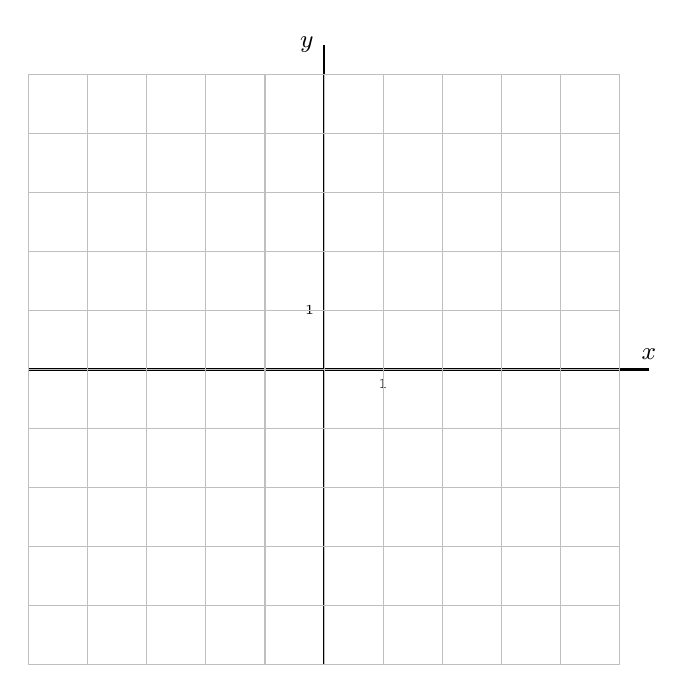
\begin{tikzpicture}[xscale=0.75,yscale=0.75]
		\draw[thick,-{\seta}] (-5,0) -- (5.5,0) node[above] {\small $x$};
		\draw[thick,-{\seta}] (0,-5) -- (0,5.5) node[left] {\small $y$};
		\draw[] (1,0) node[below] {\tiny 1};
		\draw[] (0,1) node[left] {\tiny 1};
		\draw[step=1,lightgray,thin] (-5,-5) grid (5,5);
	\end{tikzpicture}
	
	
\vfil	
	
	\item $y'=y^2$	

	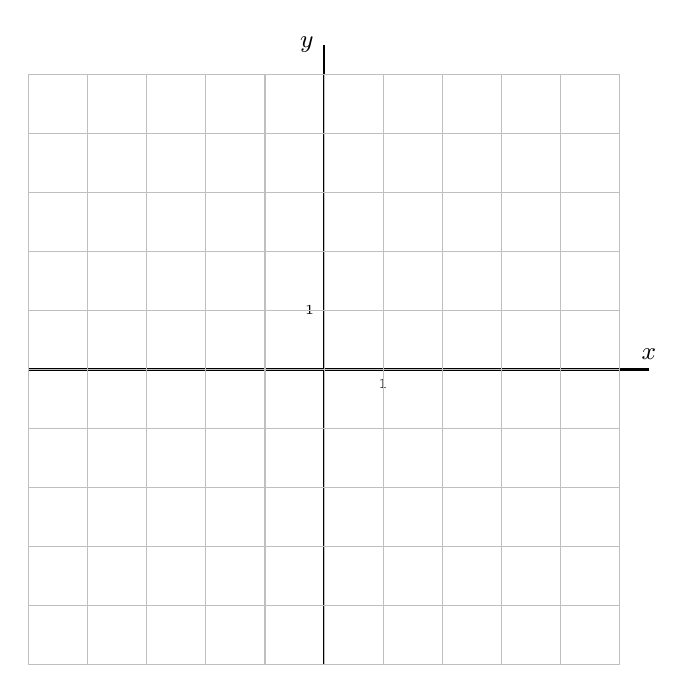
\begin{tikzpicture}[xscale=0.75,yscale=0.75]
		\draw[thick,-{\seta}] (-5,0) -- (5.5,0) node[above] {\small $x$};
		\draw[thick,-{\seta}] (0,-5) -- (0,5.5) node[left] {\small $y$};
		\draw[] (1,0) node[below] {\tiny 1};
		\draw[] (0,1) node[left] {\tiny 1};
		\draw[step=1,lightgray,thin] (-5,-5) grid (5,5);
	\end{tikzpicture}

\end{parts}



\bookonlynewpage

\question Consider the following slope fields:


\setlength{\len}{150pt}
\begin{tabular}{ccc}
	\includegraphics*[height=\len]{images/module9-graph1}
		& \includegraphics*[height=\len]{images/module9-graph2}
		& \includegraphics*[height=\len]{images/module9-graph3} \\
		(A) & (B) & (C) \\[10pt]
	\includegraphics*[height=\len]{images/module9-graph4}
		& \includegraphics*[height=\len]{images/module9-graph5}
		& \includegraphics*[height=\len]{images/module9-graph6} \\
		(D) & (E) & (F)
\end{tabular}

\hfill {\footnotesize(These slope fields were created using WolframAlpha)} \\


\begin{parts}
	\item Which slope field(s) corresponds to a differential equation of the form
		\qquad $y'=f(x)$ \qquad ?	

	\item Which slope field(s) corresponds to a differential equation of the form
		\qquad $y'=g(y)$ \qquad ?	

	\item Which slope field(s) corresponds to a differential equation of the form
		\qquad $y'=h(x+y)$ \qquad ?	

	\item Which slope field(s) corresponds to a differential equation of the form
		\qquad $y'=\kappa(x-y)$ \qquad ?	

	\item Which slope field(s) corresponds to a differential equation of the form
		\qquad $y'=1+\big( \ell(x,y) \big)^2$ \qquad ?	

	\item Which slope field(s) corresponds to a differential equation of the form
		\qquad $y'=1-\big( m(x,y) \big)^2$ \qquad ?	

\end{parts}

\begin{annotation}
	\begin{Goals}
		Students should be able to justify their choices	.
	\end{Goals}
	
\end{annotation}






\newpage




%%%%%%%%%%%%%%%%%%%%%%%%%%%%%%%%%%%%%%%%%%%%%%%%%%%%%%%%%%%%%%%%%%%%%%%%
%		Numerical Methods


\begin{module}{Numerical Methods}	
	%\Title{Numerical Methods}	
	\Heading{Objectives}
	\begin{itemize}
		\item Bla bla bla	
	\end{itemize}
	
	\Heading{Motivation} 


\end{module}





